\chapter{Foreground Component Seperation}
One of the ways of removing foregrounds from our data is to have a parametric model for the
foregrounds based on known physics and fit the data to these foreground models to get an
estimate of the parameters and use them to eliminate the foregrounds in the data. This is
the methodology followed by Commander pipeline of the Planck collaboration \cite{cmbpara} and LIL Method
\cite{lilrishi}. These methods suffer from being model dependent and the parameters are
insufficient to model the foregrounds because various physical processes
contribute to the foreground in a single pixel, making it hard to model these with a single
parametric model. Therefore, it is useful to look at
algorithms which are model independent and just use the data to estimate the foreground
characteristics.\\
Various such \emph{blind} component seperation algorithms have been proposed where
only the spectrum of the signal is needed \cite{ilc,gilc} and have been applied in various
variations such as Harmomic space, Needlet frame etc \cite{harmonicilc, needlet}. Since these
blind algorithms require the number of foreground components to be lesser than the
number of spectral channels available, it is necessary to divide the sky with similar foreground
properties into different regions and apply the algorithm seperately on those regions to reduce
the number of foreground components. These existing variations try to divide the data into
different clusters with similar foregrounds based on heuristic arguments and
our current understanding of the
properties of the foregrounds. We provide a spectral data based
approach extending upon this data driven foreground clustering approach \cite{datarishi}, which
uses the signature of the foregrounds available in the data.
Since the data is clustered only based on the spectra, different regions of the sky can still be
in the same cluster based on their foreground properties. To the best of our
knowlegde, this is the first attempt at using \emph{unsupervised} machine learning for foreground
component seperation.

\section{Generalized ILC}

\comment{Also write an appendix about the derivation of the formulas}
\section{Quick Introduction to Machine Learning}
Machine learning is a type of an algorithm which, rather than explicitly coding an algorithm for a
particular function, gives the computer the ability to \emph{learn} that function. Machine learning usually involves a
training set, from which the computer \emph{learns} the function of interest, and a validation set where the computer applies
whatever it has learned from the training set and gives us results.
Based on the way  we use our training set, machine learning can be divided into two categories.
\begin{itemize}
    \item Supervised Machine Learning
    \item UnSupervised Machine Learning
\end{itemize}

\subsection{Supervised Machine Learning}
A machine learning algorithm is said to perform supervised learning, when the training set is differet from the validation set, and we
have the expected learning outcomes as part of our training set.


\subsection{UnSupervised Machine Learning}

\subsection{Neural Networks}


\section{New tSZ maps with unsupervised Machine Learning}
\label{tSZmaps}
In unsupervised machine learning, we take the hard clustering approach,
where each data belongs only to a single class. In order to smooth the boundaries of the partitions
like the current ILC algorithms, we repeat the hard clustering multiple times with different seeds.
Since various seeds produce different partitions, and there is no a-priori reason to consider one
partition over the other, we consider all of them with equal probability. We see that this approach
essentially smoothens the boundary and no additional smoothing across the cluster boundaries are
necessary. 

\subsection{'k-means clustering' method}
\comment{EXPLAIN KMEANS}
k-means clustering partitions $n$ data points into $k$ clusters, by associating each point to the
nearest centroid, which serves as a representation of that cluster. By minimising the inertia,
We partition the space into k-regions, which serve as the partition for our clusters to be used in
ILC.
\\
\comment{INSERT IMAGE FOR KMEANS CLUSTERING HERE}
\\
The initial positions are initialized using \texttt{k-means++} algorithm inorder to avoid the
local minimas, which the random initializations can get into. And the data is rescaled with
quartile scaling, to prevent the outliers from influenzing the scaling.
k-means clustering was implemented
using \texttt{scikit-learn} \cite{scikit-learn}

\subsubsection{Choice of Variables for k-means clustering}
Let the frequency maps in $K_{CMB}$ units be denoted by, $T_i$,
where \\$i \in \{30, 44, 70, 100,143, 217, 353, 545, 857\}$Hz.
In order to model the foregrounds, We first subtract the CMB.
$A_i = T_i - T_{100Hz}$. Then we substract out the tSZ, by changing to the
corresponding $y$ units. The maps we get are mostly dominated by foregrounds.
Apart from clustering these foreground maps seperately
(labeled as \emph{raw k-means}),
we divide out the amplitudes of these \emph{raw maps} to make different measures,
which capture how fast the foreground is increasing or decreasing
with frequency similar to the measure defined in the FC-ILC (labelled as \emph{kmeans with m})
\cite{datarishi}.
\\
Let the frequency maps in $K_{CMB}$ units be denoted by, $T_i$,
where $i \in \{30, 44, 70, 100,$\\ $143, 217, 353, 545, 857\}$Hz.
In order to model the foregrounds, We first subtract the CMB.
$A_i = T_i - T_{100Hz}$. Then we substract out the tSZ, by changing to the
corresponding $y$ units.
The resultant maps we get, are dominated by foregrounds. 
\comment{EXPLAIN THESE NUMBERS - WRITE APPENDIX ON UNIT CONVERSION}
  \begin{align}
y_1 = A_{857} - 24.371 A_{143}\quad y_2 = A_{857} - 7.199 A_{217}\quad y_3 = A_{545} - 14.836 A_{143}\\
y_4 = A_{545} - 4.3826 A_{217}\quad y_5 = A_{353} - 8.215 A_{143}\quad y_6 = A_{353} - 2.4267 A_{217}\\
y_7 = A_{30} - 1.7339 A_{70}\quad y_8 = A_{44} - 1.541 A_{70}\quad y_9 = A_{217} + 3.671 A_{44}\\
y_{10} = A_{217} + 5.657 A_{70}\quad y_{11} = A_{353} + 13.73 A_{70}\quad y_{12} = A_{30} - 1.125 A_{44}\\
  \end{align}
  Apart from clustering these y-maps seperately. We divide out the amplitudes to make different
  measures, which capture how fast the foreground is increasing or decreasing with frequency.
  \begin{align}
m_1 = y_1/y_3 \quad m_2 = y_2/y_4 \quad m_3 = y_3/y_5\\
m_4 = y_4/y_6 \quad m_5 = y_7/y_{12} \quad m_6 = y_{12}/y_5\\
m_7 = y_7/y_5 \quad m_8 = y_7/y_8 \quad m_9 = y_8/y_5
  \end{align}
By visually inspecting the maps, We choose the 3 measures. $m_1, m_3, m_7$,
and perform k-means clustering.
We also masked the galactic center along with the point sources and clustered
the masked regions seperately.
\subsection{Masks}
\comment{Write about quartile scaling}
\comment{Masking the ouuliers, and deconvolving the mask using polspice when calculating the power spectrum}
\subsection{Dimensionaliy Reduction}
Since, the choice of parameters is upto us in the previous method, we use non-linear dimensionality
reduction algorithms in order to reduce the 12 dimensional input data (CMB and tSZ
substracted maps) to a lower dimension in order to
apply the k-means algorithm on it. Unlike the previous method,
we use neural networks to determine the
parameters which encode the maximum information about the data.
We use two non-linear dimensionality
reduction algorithms.\\
The two algorithms used are, 
\begin{itemize}
  \item Auto Encoders
  \item Self Organising Maps
\end{itemize}

\subsection{Auto Encoders}
We use a denoising auto encoder, made from an fully connected neural network, using $L^2$-norm as
the cost.
Once the network has been trained we can use the encoder part for dimensionality reduction.
And then the k-means algorithm is used in this lower dimensional space to cluster the pixels.
Autoencoders were implemented using \texttt{tensorflow} \cite{tensorflow}.
\subsection{Self Organising Maps}
Self organising map reduces the input data to two dimensions by fitting a discrete two dimensional
manifold on the data and then use k-means algorithm on this manifold.
Self Organising Maps was implemented using the \texttt{somoclu} Library \cite{somoclu}.

\subsection{Results}
\begin{figure}[H]
  \centering
  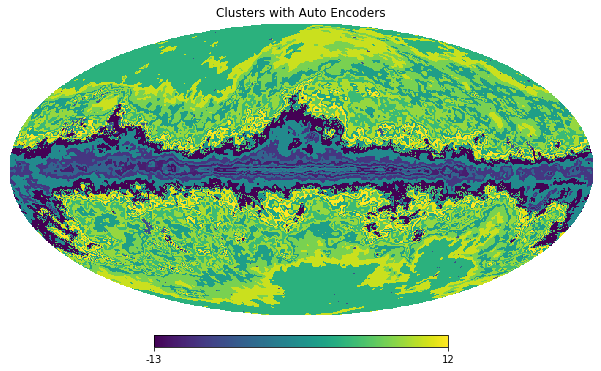
\includegraphics[width=0.35\linewidth]{auto_clusters.png}
  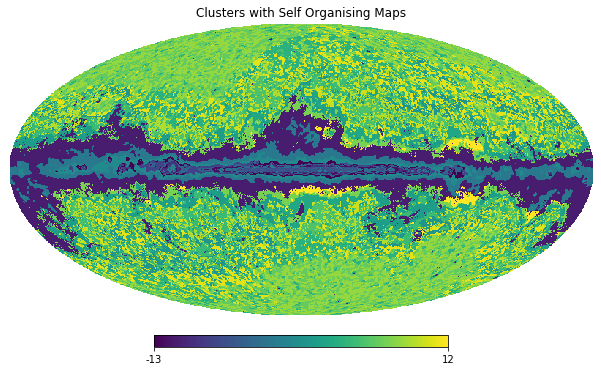
\includegraphics[width=0.35\linewidth]{som_clusters.png}
  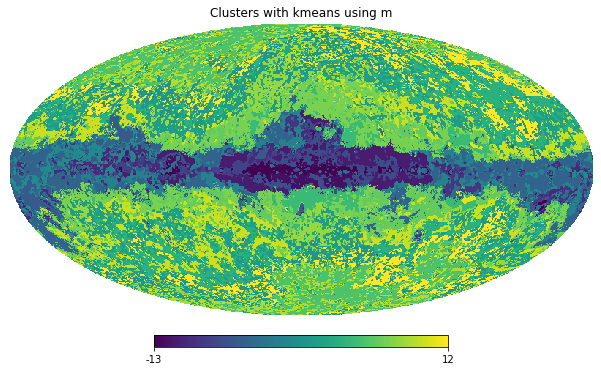
\includegraphics[width=0.35\linewidth]{kmeans_clusters.png}
  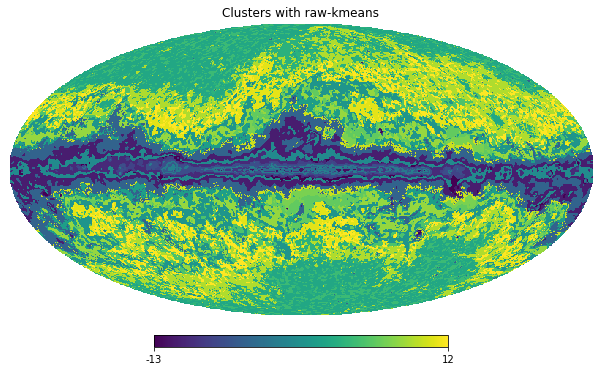
\includegraphics[width=0.35\linewidth]{raw_kmeans_clusters.png}
  \caption{A single instance Clustering of the Sky based on foregrounds using various methods (negative values indicate masked regions)}
\end{figure}



%%% Local Variables:
%%% mode: latex
%%% TeX-master: "thesis"
%%% End:
